\documentclass[titlepage]{article}
\usepackage{babel}
\usepackage{amsmath}
\usepackage{amssymb}
\usepackage{amsthm}
\usepackage{stmaryrd} %ligtning

\usepackage{tabto} %tabulator mit \tab
\usepackage{tikz}
\usetikzlibrary{automata, arrows.meta, positioning, shadows, shapes.geometric} % automaten zeichnen
\usepackage[utf8]{inputenc}
\pagestyle{plain}
\pagenumbering{arabic}
\renewcommand{\arraystretch}{1.3} %vertikaler abstand von tabellen
\usepackage[left=20mm, right=15mm, top=25mm, bottom=7mm, paper=a4paper]{geometry}

\renewcommand{\contentsname}{Inhaltsverzeichnis}
\renewcommand{\]}{\right]}
\renewcommand{\[}{\left[}
\renewcommand{\)}{\right)}
\renewcommand{\(}{\left(}
\renewcommand{\|}{\;|\;}
\newcommand{\n}{\newline}
\renewcommand{\l}{\linebreak}



\begin{document}\begingroup\let\clearpage\relax
	%header
	\begin{center}
	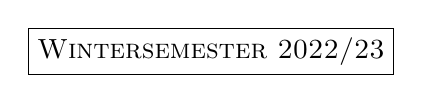
\begin{tikzpicture}
		\draw (0,0) node[draw, rectangle]{\textsc{Wintersemester 2022/23}};
	\end{tikzpicture}
	\hrulefill\\
	\begin{center}
		\LARGE\textsc{Automaten und Berechenbarkeit - Übung 05} \normalsize\\
	\end{center}
	\hrulefill
	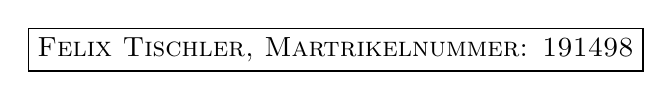
\begin{tikzpicture}
		\draw (0,0) node[draw, rectangle]{\textsc{Felix Tischler, Martrikelnummer: 191498}};
	\end{tikzpicture}
	\date{\today}
\end{center}
	
	%task one
	\paragraph{Aufgabe 1} Untersuchen Sie, ob die folgenden Sprachen über $\{a,b\}$ bzw. $\{a,b,c\}$ kontextfrei sind:
		\paragraph{(a)} $L_1=\{w\mid w\in\{a,b,c\}^*,\#_a(w)<\#_b(w)<\#_c(w)\}$
		Ann: sei $L_1\in CF\Rightarrow\exists n\in\mathbb{N}:\forall x\in L_1\;mit\;\mid x\mid\ge n:\exists x=uv_1\tilde{v}v_2w\;mit\;\mid v_1v_2\mid\ge1,\mid v_1\tilde{v}v_2\mid\le n:\forall i\in\mathbb{N}:uv_1^i\tilde{v}v_2^iw\in L_1$:
\noindent\\\\
\begin{math}
	Wähle\;x=a^nb^{n+1}c^{n+2},\;mit\\\\
	u=a^n\\
	v_1=b^{k_1}\\
	\tilde{v}=b\\
	v_2=b^{k_2}\\
	w=bc^n\\
	\;mit\;k_1+k_2=n-1\\\\
	\overset{i=0}{\Longrightarrow}a^nb^{n+1-k_1-k_2}c^{n+2}\overset{\mid v_1v_2\mid\ge1}{\Longrightarrow}L_1\notin CF
\end{math}
		\paragraph{(b)}  $L_2=\{a^nb^mc^k\mid n,m,k\in\mathbb{N},n+m=k\}$
		$G_2=(\{a,b,c\},\{S,R\},S,R)$
\begin{align*}
	Mit\;R=:
	\begin{cases}
		S&\rightarrow\quad Rc\\
		R&\rightarrow\quad aRc\mid Rbc\mid a\mid b
	\end{cases}
\end{align*} 
		\paragraph{(c)} $L_3=\{a^nb^mc^k\mid n,m,k\in\mathbb{N},n\cdot m=k\}$
		Ann: sei $L_3\in CF\Rightarrow\exists n\in\mathbb{N}:\forall x\in L_3\;mit\;\mid x\mid\ge n:\exists x=uv_1\tilde{v}v_2w\;mit\;\mid v_1v_2\mid\ge1,\mid v_1\tilde{v}v_2\mid\le n:\forall i\in\mathbb{N}:uv_1^i\tilde{v}v_2^iw\in L_3$:
\noindent\\\\
\begin{math}
	Wähle\;x=a^nb^nc^{n^2},\;mit\\\\
	u=a^{n-k_1-k_2-k_3}\\
	v_1=a^{k_1}\\
	\tilde{v}=a^{k_2}\\
	v_2=a^{k_3}\\
	w=b^nc^{n^2}\\
	mit\;k_1+k_2+k_3\le n\\\\
	\overset{i=0}{\Longrightarrow}a^{n-k_1-k_3}b^nc^{n^2}\Rightarrow L_3\notin CF
	\\\\Oder:\\\\
	u=a^n\\
	v_1=b^{k_1}\\
	\tilde{v}=b^{k_2}\\
	v_2=b^{k_3}\\
	w=c^{n^2}\\
	mit\;k_1+k_2+k_3=n\\\\
	\overset{i=0}{\Longrightarrow}a^nb^{k_2}c^{n^2}\Rightarrow L_3\notin CF
	\\\\Oder:\\\\
	u=a^nb^n\\
	v_1=c^{k_1}\\
	\tilde{v}=c^{k_2}\\
	v_2=c^{k_3}\\
	w=c^{n^2-k_1-k_2-k_3}\\
	mit\;k_1+k_2+k_3\le n\\\\
	\overset{i=0}{\Longrightarrow}a^nb^nc^{n^2-k_1-k_3}\Rightarrow L_3\notin CF
\end{math}\\
Man könnte auch noch in a und b oder in b und c pumpen, ebenso würde man durch pumpen ein nicht akzeptierbares Wort erhalten. 
		\paragraph{(d)} $A=\{0^n1^{n+m}0^m\mid n,m\in\mathbb{N},n>m>0\}$
		Ann: sei $A\in CF\Rightarrow\exists n\in\mathbb{N}:\forall x\in A\;mit\;\mid x\mid\ge n:\exists x=uv_1\tilde{v}v_2w\;mit\;\mid v_1v_2\mid\ge1,\mid v_1\tilde{v}v_2\mid\le n:\forall i\in\mathbb{N}:uv_1^i\tilde{v}v_2^iw\in A$:
\noindent\\\\
\begin{math}
	Wähle\;x=0^n1^{n+m}0^m,\;mit\\\\
	u=0^{n-k_1-k_2-k_3}\\
	v_1=0^{k_1}\\
	\tilde{v}=0^{k_2}\\
	v_2=0^{k_3}\\
	w=1^{n+m}0^m\\
	\;mit\;k_1+k_2+k_3\le n\\\\
	\overset{i=0}{\Longrightarrow}0^{n-k_1-k_3}1^{n+m}0^m\Rightarrow A\notin CF
\end{math}\\
Auch hier gibt es mehrere Möglichkeiten, wie bei (c) 
		\paragraph{(e)} $L_4=\{x\$y\mid x,y\in\{a,b\}^*,\#_a(x)=\mid y\mid\}$
		$G_2=(\{a,b\},\{S,R,K\},S,R)$
\begin{align*}
	Mit\;R=:
	\begin{cases}
		S&\rightarrow\quad aRa\mid aRb\mid bK\mid\$\\
		R&\rightarrow\quad bR\mid aRa\mid aRb\mid\$\\
		K&\rightarrow\quad aRa\mid aRb\mid bK\mid\$
	\end{cases}
\end{align*}
		\paragraph{(f)} $D=\{a^ib^jc^k\mid i,j\in\mathbb{N},i\neq j\}$
		$G_2=(\{a,b,c\},\{S,R,A,B,C\},S,R)$
\begin{align*}
	Mit\;R=:
	\begin{cases}
		S&\rightarrow\quad a\mid b\mid aRb\mid aC\mid bC\mid aA\mid bB\\
		R&\rightarrow\quad a\mid b\mid aRb\mid aC\mid bC\mid aA\mid bB\\
		A&\rightarrow\quad a\mid aA\mid aC\\
		B&\rightarrow\quad b\mid bB\mid bC\\
		C&\rightarrow\quad c\mid cC
	\end{cases}
\end{align*}
	
	\paragraph{Aufgabe 2} Konstruieren Sie einen Kellerautomaten, der die Sprache $\{w\in\{a,b\}^*\mid\#_a(w)=\#_b(w)\}$ akzeptiert.
	\begin{center}
	$M=(\{a,b\},\{A,B,\qedsymbol\},\{Z_0,Z_{ende}\},\delta,Z_0,\{Z_{Ende}\})$\\
\end{center}
Mit:
\begin{center}
	\begin{align*}
		\begin{cases}
			(Z_0,a,\qedsymbol)$&\rightarrow\quad$(Z_0,A\qedsymbol)\\
			(Z_0,a,A)$&\rightarrow\quad$(Z_0,AA)\\
			(Z_0,a,B)$&\rightarrow\quad$(Z_0,\lambda)\\
			(Z_0,\lambda,\qedsymbol)$&\rightarrow\quad$(Z_{ende})\\
			(Z_0,b,\qedsymbol)$&\rightarrow\quad$(Z_0,B\qedsymbol)\\
			(Z_0,b,A)$&\rightarrow\quad$(Z_0,\lambda)\\
			(Z_0,b,B)$&\rightarrow\quad$(Z_0,BB)
		\end{cases}
	\end{align*}
\end{center}
	
	\endgroup\end{document}